\chapter{Antriebsstrang}
\fancyfoot[C]{Lackner}


%% Übersicht %%%%%%%%%%%%%%%%%%%%%%%%%%%%%%%%%%%%%%%%%%%%%%%
\section{Übersicht}
Die Hauptaufgabe des Antriebssystems ist die Umwandlung der, vom Akkumulator zur Verfügung gestellten, elektrischen Energie in die kinetische Antriebsenergie. Diese tritt zuerst rotatorisch am Motor auf und wird zunächst über das Direkt-Getriebe umgeformt bzw. auf die passende Drehzahl gebracht, anschließend wird die Rotationsenergie mithilfe des Hinterrades auf die Straße übertragen und das ganze Motorrad beschleunigt. Neben dem Antrieb des Motorrades hat die Motorsteuerung noch weitere Bedeutung als Steuereinheit, sie fungiert als Bindeglied zwischen dem Human-Computer Interacting System und den elektrischen Anforderungen an das Gesamtsystem.


\subsection{Grundfunktionen des Systems}
Die geplanten Funktionen des Antriebssystems lassen sich grob in zwei Grundfunktionen einteilen:

\begin{itemize}
	\item \textbf{Der Antrieb} 
	\\ \medskip Translation ist eine Grundfunktion eines jeden Verkehrsmittels.
	\\ Durch die Umwandlung der elektrischen Energie in kinetische Energie erfährt 
	\\ das gesamte System eine Beschleunigung in Fahrtrichtung.
	\medskip
	\item \textbf{Die Steuereinheit}
	\\ \medskip Steuerung und Kommunikation mit anderen Betriebsmitteln.
	\\ Realisiert durch In- und Outputs, Datenübetragung mithilfe des CAN-Buses. 
\end{itemize}

\vspace{5mm}

Um auf die einzelnen Details des Antriebssystems besser eingehen zu können, unterscheiden wir zwischen dem Hardwareaufbau und dem Softwareaufbau des Antriebssystems.

\newpage



%% Hardwareaufbau %%%%%%%%%%%%%%%%%%%%%%%%%%%%%%%%%%%%%%%%%%%%%%%
\section{Hardwareaufbau des Antriebssystems}
Der grundsätzliche Hardwareaufbau des Antriebssystems lässt sich in zwei galvanisch getrennte Stromkreise und der mechanischen Umsetzung unterscheiden:
\\[5mm]
\begin{itemize}
	\item \textbf{Mechanische Umsetzung (Kraftübertragung und Montage)} 
	\\ \medskip Umfasst das Getriebe und die Befestigung aller Komponenten am Rahmen.
	\medskip
	\item \textbf{Der Laststromkreis}
	\\ \medskip Beinhaltet die Verbindung des Motorcontrollers mit dem Motor und dem Akkumulator.
	\medskip
	\item \textbf{Der Steuerstromkreis}
	\\ \medskip Beinhaltet alle elektrischen Verbindungen, welche mithilfe des 35-poligen
	\\ Niederleistungs-Steckers mit dem Motorcontroller verbunden sind.
\end{itemize}

\newpage



%% Mechanische Umsetzung %%%%%%%%%%%%%%%%%%%%%%%%%%%%%%%%%%%%%%%%%%%%%%% 
\subsection{Mechanische Umsetzung}
Die Fertigung des Getriebes und die Montage der einzelnen Betriebsmittel wurde vollständig von Tobias Schmeisser übernommen.


\newpage



%% Der Laststromkreis %%%%%%%%%%%%%%%%%%%%%%%%%%%%%%%%%
\subsection{Der Laststromkreis}
Der Laststromkreis beinhaltet allen leistungsführenden Betriebsmitteln des Antriebssystems. Hierbei unterscheiden wir zwischen den zwei wichtigsten Grundfunktionen:
\\[5mm]
\begin{itemize}
	\item \textbf{Elektrische Energieübertragung}
	\\ \medskip Umfasst die elektrische Verbindung von Motor, Motorcontroller und Akkumulator. 			\\ Realisiert durch einfache Leitungen, um Leistungen übertragen zu können.
	\medskip
	\item \textbf{Schutz der Komponenten vor Beschädigungen (Leitungsschutzorgane)}
	\\ \medskip Beinhaltet eine Schmelzsicherung zum Schutz vor Überströmen und ein 					\\ Hochleistungs-Relais, um im Fehlerfall den Laststromkreis öffnen zu können und damit eine  		
	\\ galvanische Trennung des Antriebs und der Energieversorgung gewährleisten zu können.
\end{itemize}

\begin{figure}[H]
	\begin{center}
		%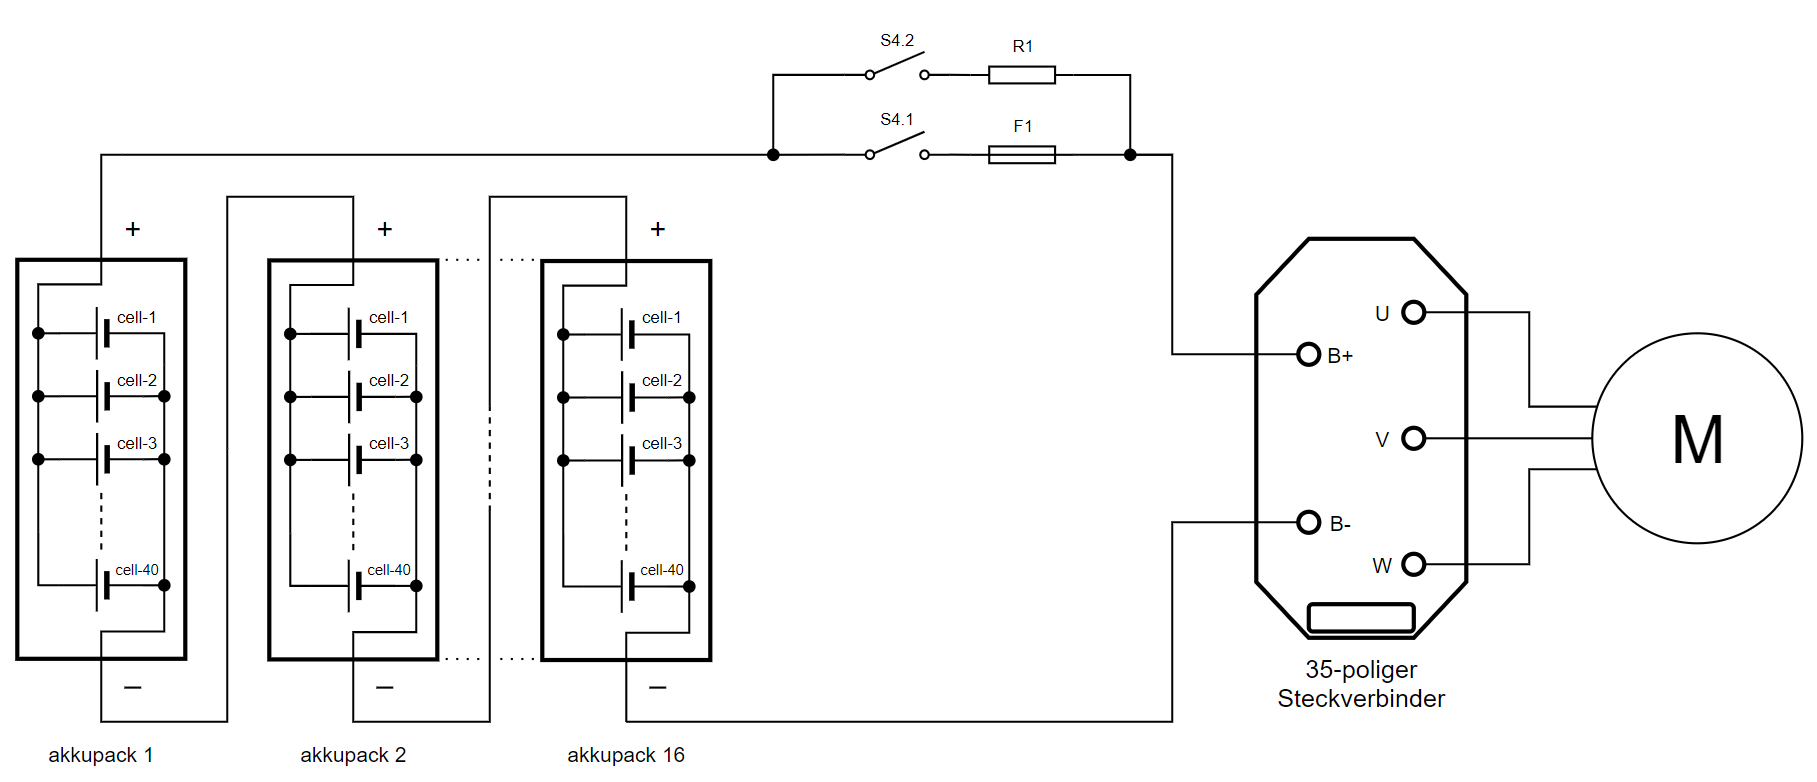
\includegraphics[scale=0.5]{figures/hcis/Antrieb_Laststromkreis.png}
		\caption{Grundaufbau des Laststromkreises}
	\end{center}
\end{figure}

\newpage



%% Elektrische Energieübertragung %%%%%%%%%%%%%%%%%%%%%%%%%%%%%%%%%
\subsubsection{Elektrische Energieübertragung}
Um die benötigte elektrische Energie übertragen zu können, müssen die Leitungen an den Leistungsverbrauch des Verbrauchers (Motor) angepasst werden. Bei einer zu hohen Stromaufnahme (Überlast) des Motors kann es zu einer übermäßigen Erwärmung der Leitungen bis hin zu dauerhaften Beschädigungen, wie Durchschmoren der Isolierung, oder sogar einen Leitungsbrand führen. Um dies verhindern zu können, müssen die Leitungen an die Stromaufnahme des Motors angepasst werden. Das heißt, der zulässige Dauerstrom der Leitungen muss den maximalen Dauerstrom des Motors bzw. den maximalen Dauerstrom, welcher durch den Akkumulator zur Verfügung gestellten werden kann, übersteigen.
\\[5mm]

\textbf{Berechnung:} 
\\[2mm]
In diesem Abschnitt befassen wir uns zunächst mit der Berechnung aller Ströme, die wir zur Auswahl der richtigen Leitungen benötigen. Bei der Auswahl von Leitungen muss man grundsätzlich den Querschnitt und die Länge der Leitung an die benötigte Stromaufnahme des Motors anpassen.

Anzahl der Zellen die parallel verschaltet werden: 40


\begin{align*}
I_{Zmax} &= 14~\mathrm{A}	\\
I_{max} &= 40 \cdot I_{Zmax} = 40 \cdot 14~\mathrm{A} = 560~\mathrm{A}
\end{align*}
%
% 	 \nonumber	\\

% 	 	\\
%R = \dfrac{\delta \cdot l}{A} = \frac{0,0278~\mathrm{\dfrac{\Omega \cdot mm^{2}}{m}}  \cdot 1~\mathrm{m}{70\mathrm{mm^{2}}}}  	\\

%

%\Delta U &=\frac{•}{•}

%\\[5mm]

\textbf{Auswahl:}
\\[2mm]
text
\\[5mm]

\textbf{Fazit:}
\\[2mm]
text

\newpage



%% Leitungsschutzorgane %%%%%%%%%%%%%%%%%%%%%%%%%%%%%%%%%
\subsubsection{Leitungsschutzorgane}
Die Aufgabe der Leitungsschutzorgane ist es, bei unerwarteten Überströmen oder in einem Fehlerfall den Laststromkreis zu öffnen, um damit den Motor bzw. Motorcontroller vom Akkumulator galvanisch zu trennen. Diese Maßnahme wird ergriffen, um mögliche Beschädigungen an den Komponenten oder an den Leitungen verhindern zu können. Da jedoch ungewünschte Fehlauslösungen zum sofortigen Stillstand des Motorrades führen und eventuell sogar benötigte Wartungen (Wechsel der durchgebrannten Schmelzsicherung) nach sich ziehen, müssen diese Leitungsschutzorgane sehr sorgfältig ausgewählt werden. Eine Überdimensionierung ist ebenso unerwünscht, denn dadurch steigen die Anschaffungskosten der Bauteile. Das noch größere Problem entsteht jedoch bei der Überdimensionierung der Schmelzsicherung, denn diese löst nun zu spät aus und hat damit nur mehr eine sehr geringe bis gar keine Schutzfunktion. 

\textbf{Berechnung:} 
\\[2mm]
text
\\[5mm]

\textbf{Auswahl:}
\\[2mm]
text
\\[5mm]

\textbf{Fazit:}
\\[2mm]
text

\newpage



%% Der Steuerstromkreis %%%%%%%%%%%%%%%%%%%%%%%%%%%%%%%%%%%%%%%%%%%%%%%
\subsection{Der Steuerstromkreis}
\subsubsection{Übersicht Ein- und Ausgänge}
Der Steuerstromkreis befasst sich mit allen elektrischen Verbindungen, welche über den  35-poligen Niederleistungs-Stecker mit dem Motorcontroller verbunden sind. Hierbei unterscheiden wir grundsätzlich zwischen drei verchiedenen Ports, welche nochmals unterkategorisiert werden können:

\vspace{3mm}

\begin{itemize}
	\item \textbf{Eingänge (Inputs)}
	\\ - Digitale Eingänge (Digital Inputs)
	\\ - Analoge Eingänge (Analog Inputs)
	\\ - Gas- und Bremseingänge (Throttle and Brake Inputs)
	\\ - Positionsrückmeldung vom Encoder (Position-feedback Input)
	\\ - Prozessorversorgung und Spulenrücklauf (KSI and Coil Return)
	\item \textbf{Ausgänge (Outputs)}
	\\ - Analoge Ausgänge (Analog Outputs)
	\\ - Digitale und Pulsweitenmodulierbare Ausgänge (Digital and PWM Outputs)
	\\ - Spannungsversorgungs-Ausgänge (Power Supply Outputs)
	\item \textbf{Kommunikation (Communication)}
	\\ -  CAN-Bus (CAN-Port)
	\\ -  Serielle Schnittstelle (Serial-Port)
\end{itemize}

\vspace{5mm}

Der Motorcontroller verfügt über viele Pins, welche über mehrere Funktionen verfügen, es muss jedoch eine dieser Funktionen ausgewählt werden. Pin 6 zum Beispiel wird eigentlich als digitaler und phasenmodulierbarer Ausgang verwendet, bei richtiger Konfiguration kann er jedoch auch als digitaler Input verwendet werden. Weiteres kann frei konfiguriert werden, ob man mit diesem Ausgang zum Beispiel das Hochleistungs-Relais oder einen Spannungswandler ansteuern möchte. Um den passenden Pin für eine Anwendung auswählen zu können, muss man jedoch die elektrischen Eigenschaften der Pins genauer unter die Lupe nehmen. Oftmals haben auch die Pins der selben Unterkategorie verschiedene Funktionen, Eingangsimpedanzen oder Toleranzen. 

\begin{figure}[H]
	\begin{center}
		%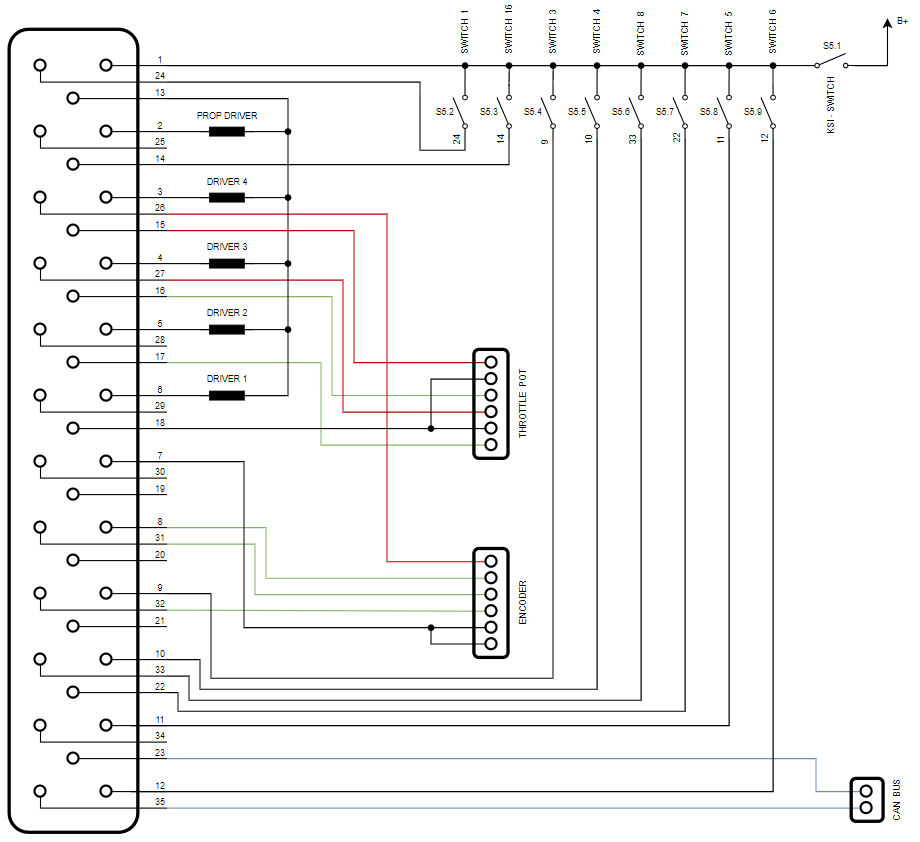
\includegraphics[scale=0.5]{figures/hcis/Antrieb_Steuerstromkreis.png}
		\caption{Grundaufbau des Steuerstromkreises}
	\end{center}
\end{figure}

\newpage



%% Digitale Eingänge (Digital Inputs) %%%%%%%%%%%%%%%%%%%%%%%%%%%%%%%%%%%%%%%%%%%%%%%
\subsubsection{Digitale Eingänge (Digital Inputs)}
Es gibt insgesamt 16 Pins, die als digitale Eingänge genutzt werden können, jedoch werden sieben Pins davon eigentlich als Ausgänge konfiguriert. 

\begin{figure}[H]
	\begin{center}
		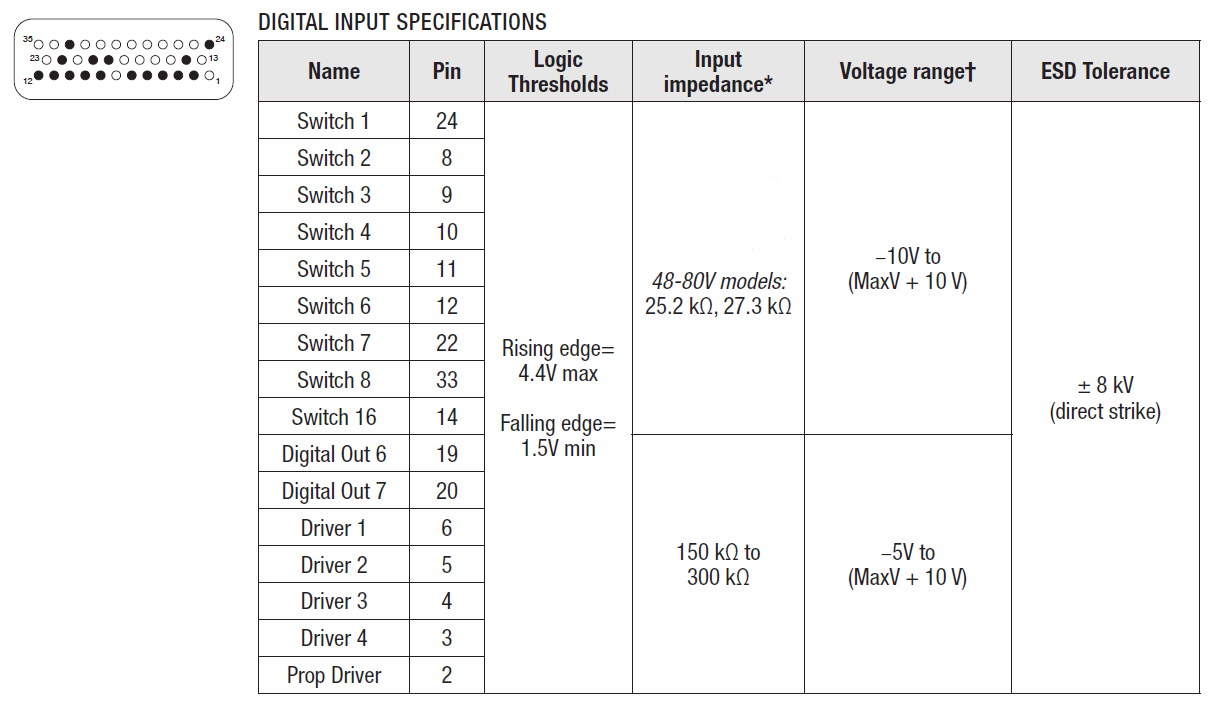
\includegraphics[width=\textwidth]{figures/antrieb/Digital_Input_Specifications.png}
		\caption{Digital Input Specifications}
	\end{center}
\end{figure}




%% Analoge Eingänge (Analog Inputs) %%%%%%%%%%%%%%%%%%%%%%%%%%%%%%%%%%%%%%%%%%%%%%%
\subsubsection{Analoge Eingänge (Analog Inputs)}
Es gibt insgesamt zwei Pins die als analoge Eingänge verwendet werden können. Ein Pin davon wird jedoch im Normalfall für den Motortemperatur-Sensor verwendet. Die Eingänge, die für das Gas- und Bremspotentiometer verwendet werden, sind in dieser Kategorie nicht aufgelistet, obwohl diese ebenfalls als analoge Eingänge genutzt werden. Diese Pins sind jedoch speziell für die Gas- und Bremssteuerung konfiguriert und sollten im Normalfall auch dafür hergenommen werden.

\begin{figure}[H]
	\begin{center}
		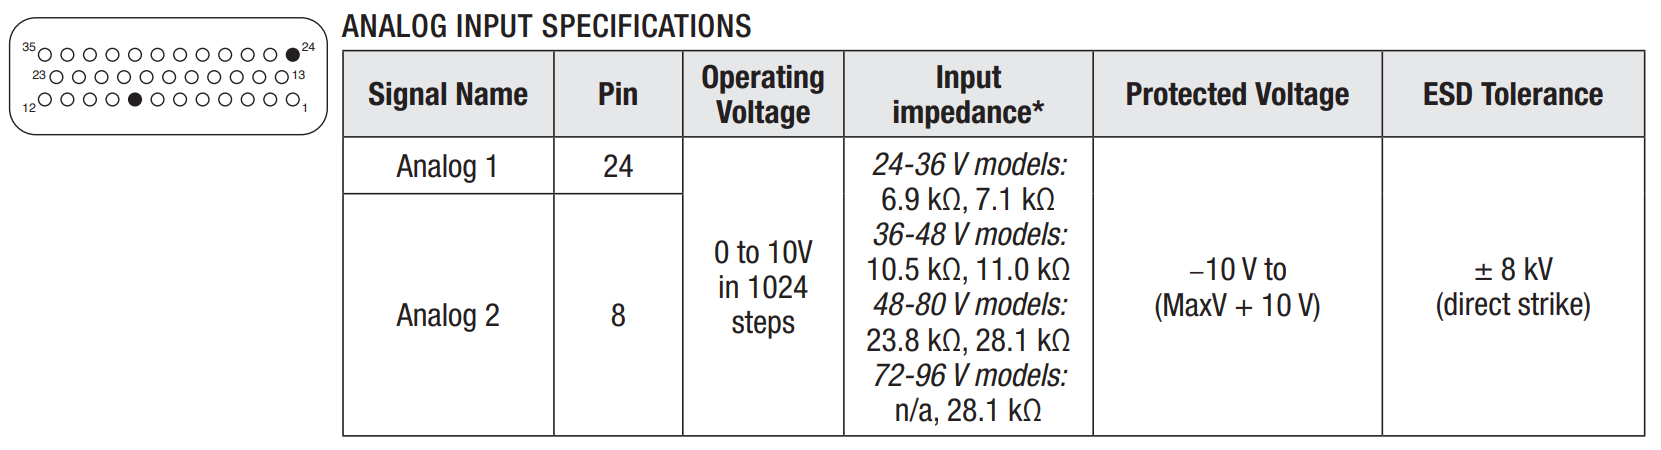
\includegraphics[width=\textwidth]{figures/antrieb/Analog_Input_Specifications.png}
		\caption{Analog Input Specifications}
	\end{center}
\end{figure}



\newpage



%% Gas- und Bremseingänge (Throttle and Brake Inputs) %%%%%%%%%%%%%%%%%%%%%%%%%%%%%%%%%%%%%%%%%%%%%%%
\subsubsection{Gas- und Bremseingänge (Throttle and Brake Inputs)}
Die zwei Gas- oder Bremssteuerungs-Eingänge können unabhängig voneinander programmiert werden. Sie sind optimiert für die Anwendung mittels Spannungssteuerung, 2-Draht Widerstandssteuerung oder 3-Draht Widerstandssteuerung. Bei der Spannungssteuerung benötigt man die Pins Pot Wiper und I/O Ground, bei der 2-Draht Widerstandssteuerung Pot Wiper und Pot Low und bei der 3-Draht Widerstandssteuerung Pot High, Pot Wiper und Pot Low. In unserem Fall benutzen wir beide Steuerungs-Eingänge für die 3-Draht Widerstandssteuerung, da der Gasdrehgriff über eine Drahtbrucherkennung verfügt. Das heißt, der Gasdrehgriff hat insgesamt zwei unabhängige 3-Draht Potentiometer-Ausgänge, welche beide für den Gaseingang benutzt werden.

\begin{figure}[H]
	\begin{center}
		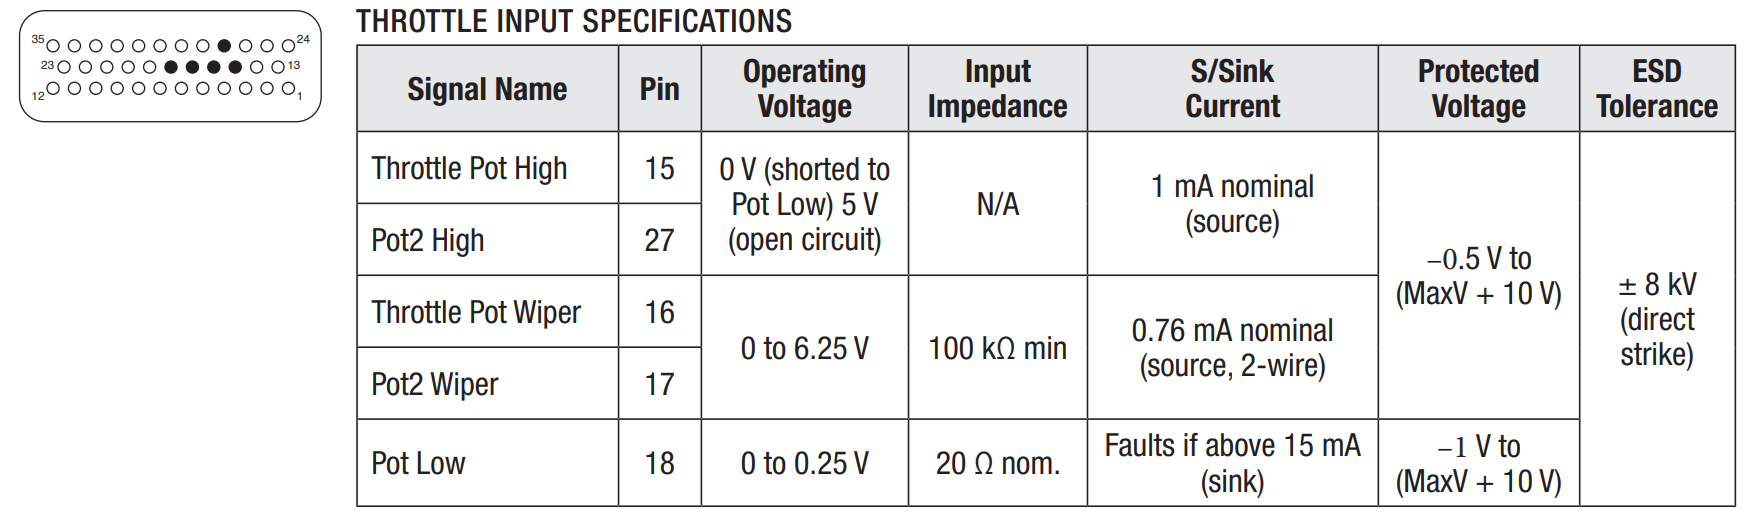
\includegraphics[width=\textwidth]{figures/antrieb/Throttle_Input_Specifications.png}
		\caption{Throttle Input Specifications}
	\end{center}
\end{figure}



%% Positionsrückmeldung vom Encoder (Position-feedback Input) %%%%%%%%%%%%%%%%%%%%%%%%%%%%%%%%%%%%%%%%%%
\subsubsection{Positionsrückmeldung vom Encoder (Position-feedback Input)}
Diese zwei Pins sind intern dafür konfiguriert, die aktuelle Position der Motorwelle einzulesen, um eine optimale feldorienterte Ansteuerung des Motors durchführen zu können. Dabei gibt es die Möglichkeiten über einen Quadratur-Encoder oder einen Sin/Cos-Encoder. Da im Ashwoods-Motor ein Sin/Cos-Sensor verbaut ist, wurde dies vorab beim Motorcontroller eingestellt.

\begin{figure}[H]
	\begin{center}
		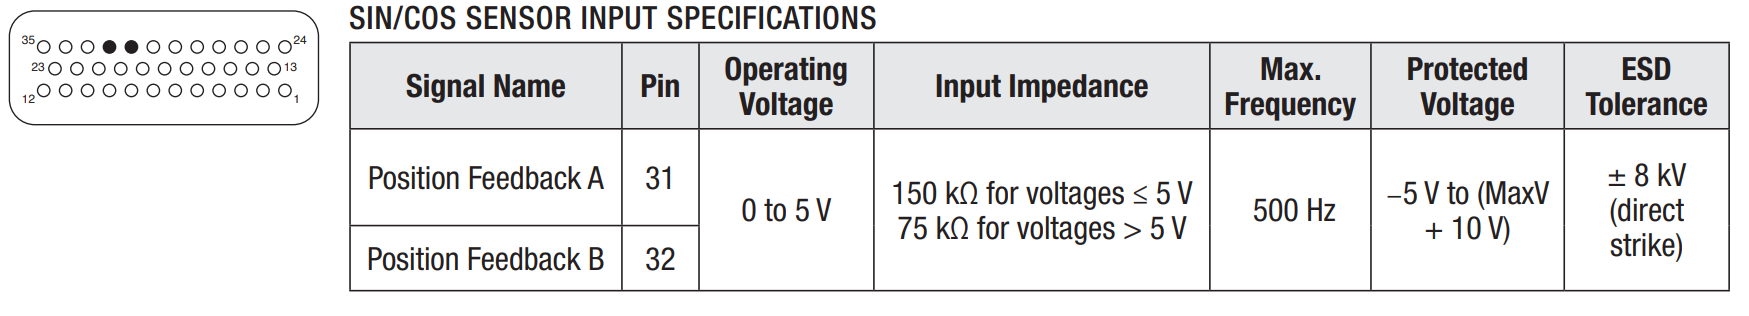
\includegraphics[width=\textwidth]{figures/antrieb/SinCosSensor_Input_Specifications.png}
		\caption{Sin/Cos Sensor Input Specifications}
	\end{center}
\end{figure}


\newpage


%% Prozessorversorgung und Spulenrücklauf (KSI and Coil Return) %%%%%%%%%%%%%%%%%%%%%%%%%%%%%%%%%%%%%%
\subsubsection{Prozessorversorgung und Spulenrücklauf (KSI and Coil Return)}
Der KSI-Eingang stellt die elektrische Versorgung aller Niederleistungs-Schaltkreise zur Verfügung. Dies  beinhaltet ebenfalls die Versorgung aller Ausgänge und die Kondensator-Vorlade-Funktion, welche dazu dient, die Kondensatoren vorzuladen, um hohe Einschaltströme zu verhindern. Der Spulenrücklauf stellt die Versorgung der pulsweitenmodulierbaren Ausgänge zur Verfügung und hat die gleiche Spannung wie der KSI-Pin. Er soll übermäßige Schaltgeräusche im PWM-Betrieb verhindern und nur auf die Spulen begrenzen. Die elektrische Trennung von KSI und Coil Return muss aufrechterhalten werden, um einen Verpolungsschutz gewährleisten zu können. 

\begin{figure}[H]
	\begin{center}
		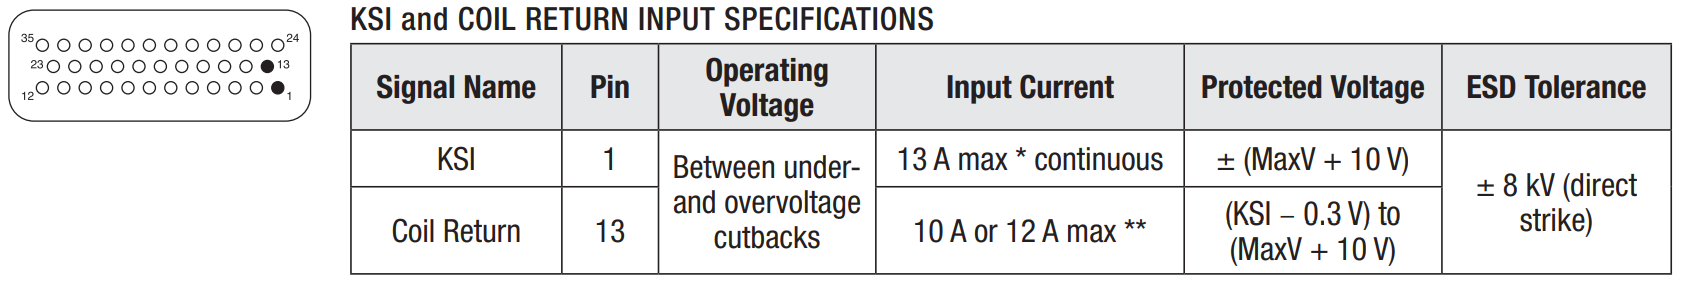
\includegraphics[width=\textwidth]{figures/antrieb/KSI_CoilReturn_Input_Specifications.png}
		\caption{KSI and Coil Return Input Specifications}
	\end{center}
\end{figure}



%% Analoge Ausgänge (Analog Outputs %%%%%%%%%%%%%%%%%%%%%%%%%%%%%%%%%%%%%%%%%%%%%%%
\subsubsection{Analoge Ausgänge (Analog Outputs)}
Der analoge Ausgang kann ein Spannungssignal von 0 bis 10V ausgeben. Dieser Ausgang ist für die Ausgabe über Anzeigeinstrumente, wie zum Beispiel eine Anzeige über den aktuellen Ladestand des Akkumulators, vorgesehen.

\begin{figure}[H]
	\begin{center}
		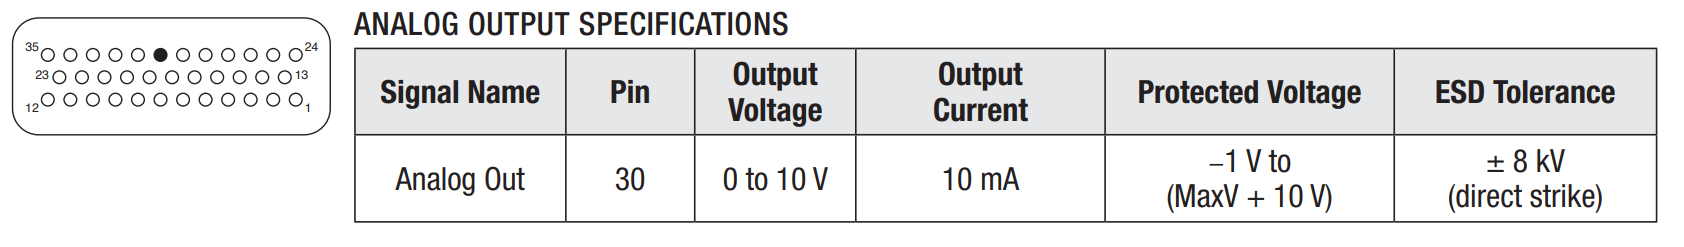
\includegraphics[width=\textwidth]{figures/antrieb/Analog_Output_Specifications.png}
		\caption{Analog Output Specifications}
	\end{center}
\end{figure}


\newpage



%% Digitale und Pulsweitenmodulierbare Ausgänge (Digital and PWM Outputs) %%%%%%%%%%%%%%%%%%%%%%%%%%%%
\subsubsection{Digitale und Pulsweitenmodulierbare Ausgänge (Digital and PWM Outputs)}
Es gibt insgesamt 7 digitale Ausgänge, wovon jedoch nur 5 für eine Pulsweitenmodulation konfiguriert werden können. Diese Ausgänge sind für induktive Lasten, wie zum Beispiel den Hauptschütz oder eine elektromagnetische Bremse, vorgesehen. Rein ohmsche Lasten können ebenfalls gesteuert werden, jedoch darf der zulässige Spitzenstrom nicht überschritten werden. Der Proportional-Driver kann bei richtiger Konfiguration auch für die Anzeige eines Tachometers hergenommen werden. Generell kann jeder Pin dieser Gruppe ebenfalls als digitaler Eingang benutzt werden.

\begin{figure}[H]
	\begin{center}
		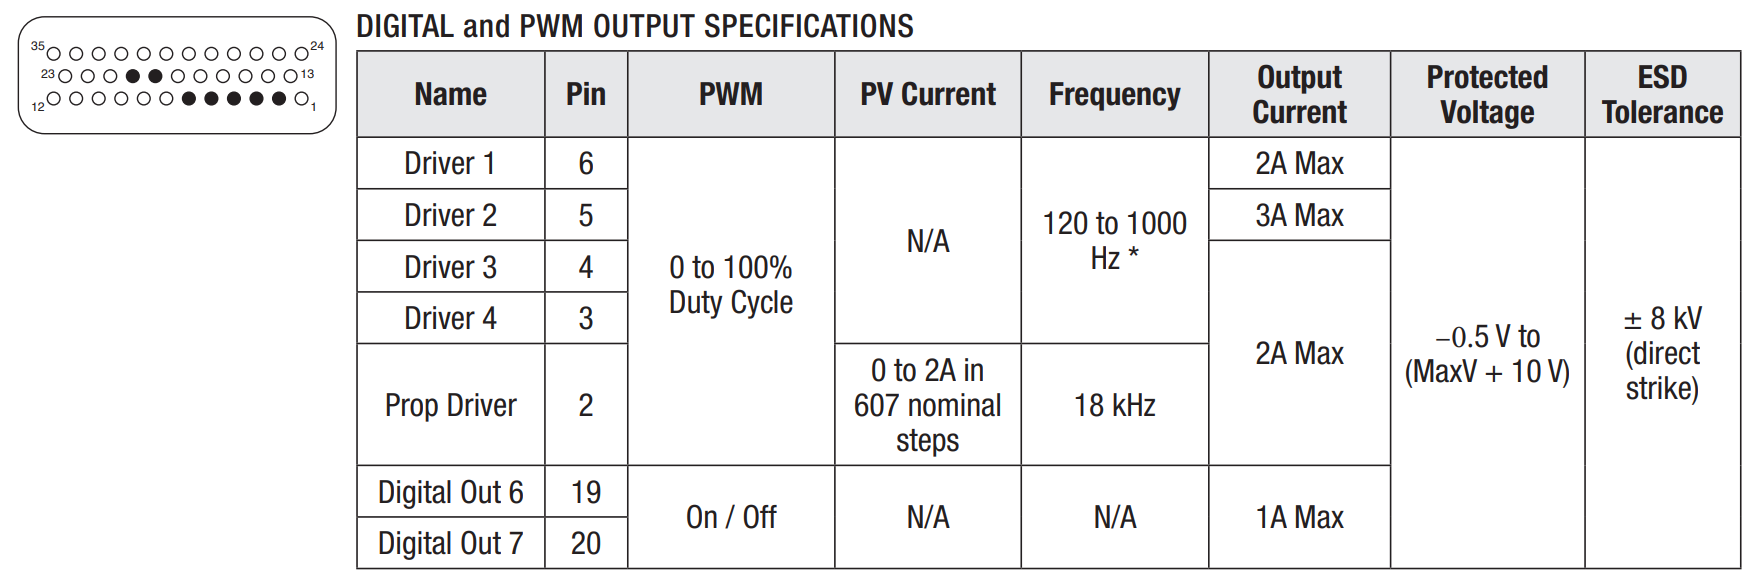
\includegraphics[width=\textwidth]{figures/antrieb/Digital_PWM_Output_Specifications.png}
		\caption{Digital and PWM Output Specifications}
	\end{center}
\end{figure}



%% Spannungsversorgungs-Ausgänge (Power Supply Outputs) %%%%%%%%%%%%%%%%%%%%%%%%%%%%%%%%%%%%%%%%%%%%%%
\subsubsection{Spannungsversorgungs-Ausgänge (Power Supply Outputs)}
Um kleine Schaltkreise, wie zum Beispiel einen LED-Indikator oder die Positionsrückmeldung vom Encoder, mit Spannung versorgen zu können, gibt es zwei dafür vorgesehene Spannungsversorgungs-Ausgänge mit einem Pin für 5V und 12V. Für diese Anwendungen gibt es ebenfalls noch einen Rücklauf, der als I/O Ground definiert wurde.

\begin{figure}[H]
	\begin{center}
		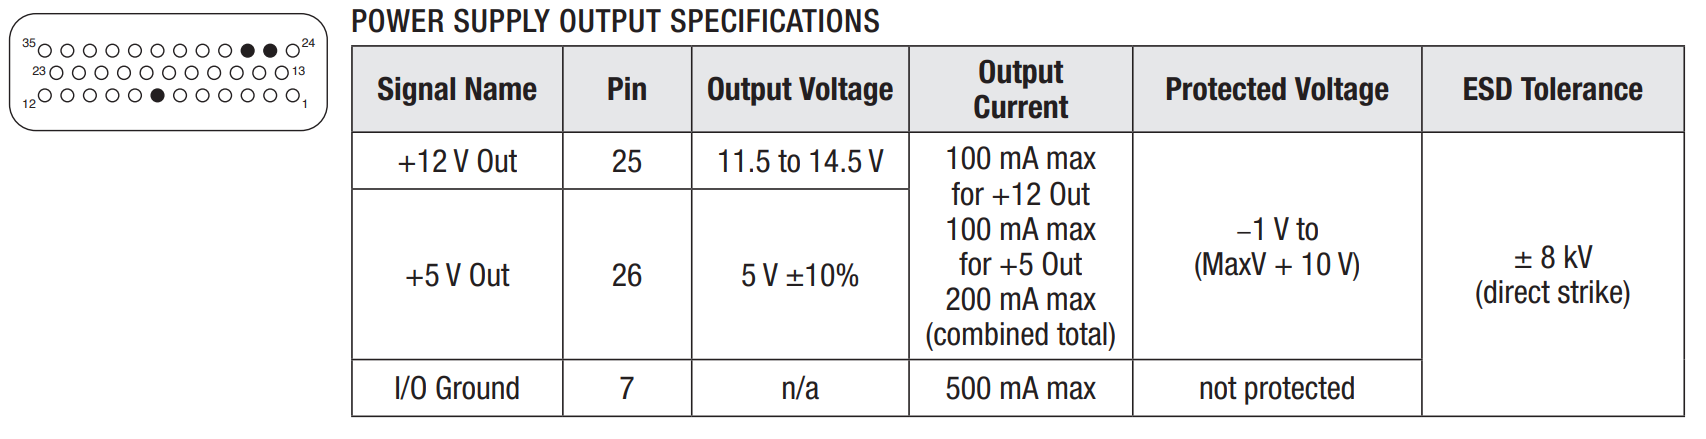
\includegraphics[width=\textwidth]{figures/antrieb/Power_Supply_Output_Specifications.png}
		\caption{Power Supply Output Specifications}
	\end{center}
\end{figure}


\newpage


%% Kommunikations-Ports %%%%%%%%%%%%%%%%%%%%%%%%%%%%%%%%%%%%%%%%%%%%%%%
\subsubsection{Kommunikations-Ports}
Für die Kommunikation mit anderen Betriebsmitteln stellt uns der Motorcontroller zwei Möglichkeiten zur Verfügung, den CAN-Bus und die serielle Schnittstelle. Da sich unser Projektteam auf die Nutzung des CAN-Busses geeinigt hat, wird die serielle Schnittstelle nicht verwendet. Die zwei Pins CAN Term High und CAN Term Low werden ebenfalls nicht benötigt, denn diese dienen nur dazu, den CAN-Bus vorübergehend funktionsunfähig zu schalten. Programmtechnisch gibt es drei Möglichkeiten zur Konfiguration des CAN-Busses, dies wird jedoch im Punkt Software genauer erklärt.

\begin{figure}[H]
	\begin{center}
		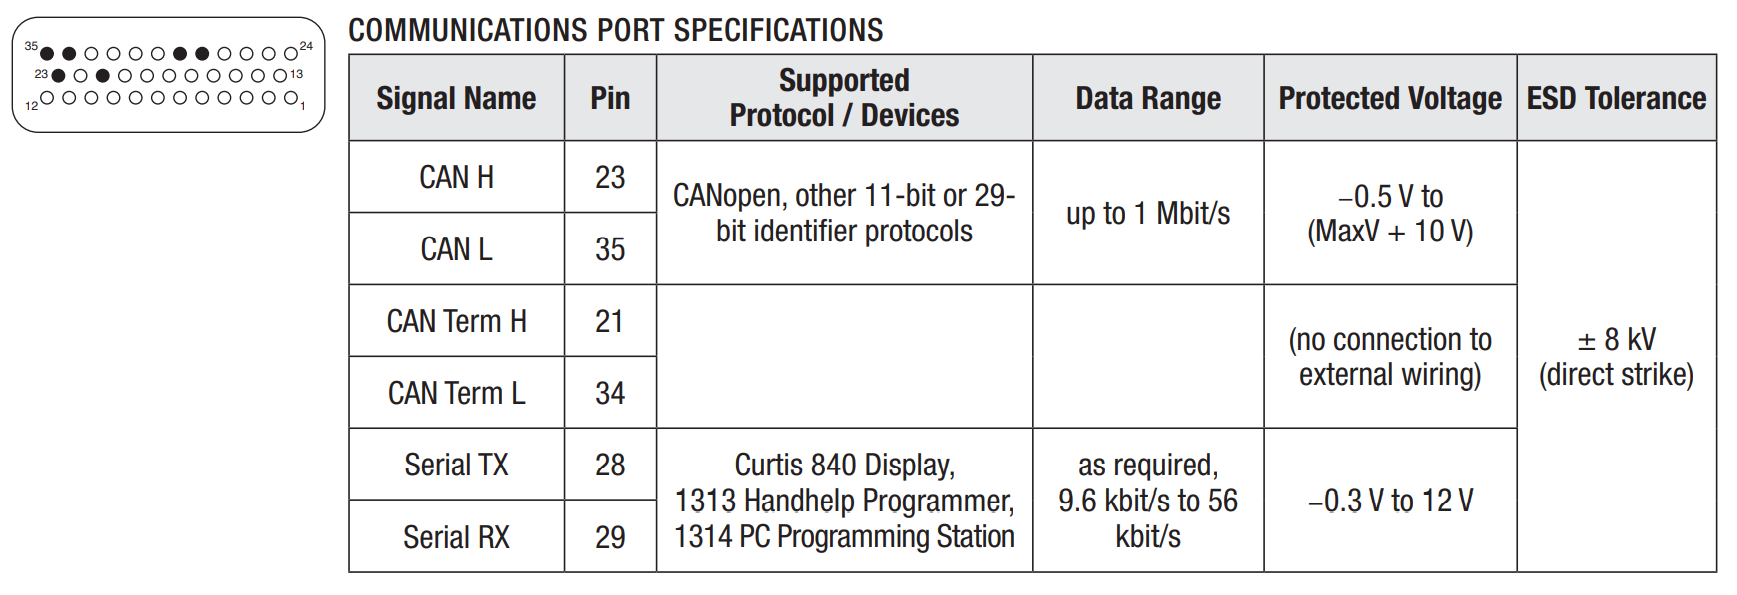
\includegraphics[width=\textwidth]{figures/antrieb/Communications_Port_Specifications.png}
		\caption{Communications Port Specifications}
	\end{center}
\end{figure}



\newpage



%% Softwareaufbau %%%%%%%%%%%%%%%%%%%%%%%%%%%%%%%%%%%%%%%
\section{Softwareaufbau des Antriebssystems}
Der Softwareaufbau des Antriebssystems kann grob in 3 Grundfunktionen unterteilt werden:
\\[5mm]
\begin{itemize}
	\item \textbf{Steuerung der Ein- und Ausgänge (I/O Assignment)}
	\\ \medskip Umfasst alle Parameter und die vornehmbaren Konfigurationsmöglichkeiten.
	\medskip
	\item \textbf{Drehmomentsteuerung (Torquecontrol)}
	\\ \medskip Beinhaltet alle Parametereinstellungen, welche für die Drehmomentsteuerung ausschlaggebend sind.
	\medskip
	\item \textbf{Vehicle-Control-Language (VCL) Programmierung}
	\\ \medskip Umfasst das gesamte Programm, welches mit der Vehicle-Control-Language realisiert wurde.
	\\ Ein Großteil dieses Programms beschäftigt sich hierbei mit der Kommunikation mit dem Raspberry PI.
\end{itemize}

%% Steuerung der In- und Outputs %%%%%%%%%%%%%%%%%%%%%%%%%%%%%%%%%%%%%%%%%%%%
\subsection{Steuerung der Ein- und Ausgänge (I/O Assingment)}

\subsubsection{Funktionen}
\subsubsection{Zuweisung}

\newpage

%% Drehmomentsteuerung %%%%%%%%%%%%%%%%%%%%%%%%%%%%%%%%%%%%%%%%%%%%
\subsection{Drehmomentsteuerung (Torquecontrol)}
Die Drehmomensteuerung wird mithilfe von 12 unterschiedlichen Parametern beschrieben. Generell können diese Parameter eher als Feineinstellungen angesehen werden, da der grundsätzliche Vorgang immer der gleiche bleibt. Mit diesen Parametern werden jedoch die maximale Geschwindigkeit, die Reaktionszeit und die Aggresivität des Motors genau definiert, um das gewünschte Beschleunigungsmuster erhalten zu können.

\vspace{5mm}
 
\subsubsection{Parameter}
Grundsätzlich lassen sich diese Parameter in zwei Hauptgruppen unterscheiden:
\\[5mm]
\begin{itemize}
	\item \textbf{Geschwindigkeitsbegrenzer-Parameter (Speed-Limiter)}
	\\ \medskip Bestimmen die maximale Geschwindigkeit und die Begrenzungsparameter des KPI-Reglers.
	\medskip
	\item \textbf{Reaktions-Parameter (Response)}
	\\ \medskip Bestimmen die verschiedensten Ansprechzeiten und Drehzahlen für bestimmte Ereignisse.
\end{itemize}

\vspace{5mm}

Diese Parameter werden in den folgenden Tabellen noch genau erklärt:

\vspace{5mm}

\setlength{\tabcolsep}{9pt}
\begin{table}[H]
	\begin{tabular}{|lcp{8cm}|}\hline
	\rowcolor[gray]{0.8}\textbf{Parameter} & \textbf{Einstellungsbereich} &\textbf{Beschreibung}\\[2pt]
		Max Speed 	& 500-8000 U/min 	& Definiert die maximale Geschwindigkeit in U/min, welche mittels der Drehmomentsteuerung angesteuert werden kann. (Unabhängig von der Gasdrehgriff-Stellung)\\\hline
		Kp 			& 0 – 100 \% 		& Legt fest, wie aggressiv der Drehzahlregler versucht, die Motordrehzahl auf die maximale Drehzahl zu begrenzen. Größere Werte sorgen für eine genauere Kontrolle, können jedoch zu Schwankungen führen. Bei einem zu niedrigen Kp kann die maximal Geschwindigkeit den Parameter Max Speed überschreiten.\\\hline
		Ki 			& 5 – 100 \% 		& Mit diesem Parameter kann die Integralregelung genauer beschrieben werden, welche die Drehzahlbegrenzung unterschiedlich stark beeinflusst, abhängig von der aktuellen Regelabweichung. Größere Werte ermöglichen eine schnellere Regelung, können jedoch zu Schwankungen führen. Bei zu niedrigen Werten kann es lange dauern, bis sich der Motor bei einer Überdrehzahl dem Max Speed nähert. \\\hline
		Kd    		& 0 – 100 \% 		& Beschreibt die Dämpfung, wenn sich das Fahrzeug der Höchstgeschwindigkeit nähert, dadurch werden Überschwingungen verringert. Bei einem zu hohen Kd kann es lange dauern, bis die Höchstgeschwindigkeit erreicht wird. Wenn Kd zu niedrig eingestellt ist, kann die Höchstgeschwindigkeit überschritten werden, insbesondere beim bergab Fahren. \\\hline		
	\end{tabular}	
	\caption{Geschwindigkeitsbegrenzer-Parameter}
	\label{tab:Geschwindigkeitsbegrenzer-Parameter}
\end{table}

\newpage

\setlength{\tabcolsep}{6pt}
\begin{table}[H]
	\begin{tabular}{|p{2.5cm}cp{8cm}|}\hline
	\rowcolor[gray]{0.8}\textbf{Parameter} & \textbf{Einstellungsbereich} &\textbf{Beschreibung}\\[2pt]
		Accel Rate 						& 0.1 - 30.0 s 		& Legt fest, wie lange es dauert, bis das Motordrehmoment bei Vollgas auf das Maximum angestiegen ist. Größere Werte bedeuten eine langsamere Reaktion. \\\hline
		Accel Release Rate				& 0.1 - 2.0 s 	 	&  Legt fest, wie schnell die Verzögerung des Fahrzeugs bei einem loslassen des Gasdrehgriffs eingeleitet wird. Bei einem geringen Wert wird der Übergang abrupt eingeleitet. Ist der Wert zu hoch eingestellt, fährt das Fahrzeug für kurze Zeit weiter.\\\hline
		Brake Rate 						& 0.1 - 5.0 s 	 	& Legt fest, wie lange es dauert, bis das Bremsmoment bei einem startenden Bremsvorgang oder einem Fahrtrichtungswechsel aufgebaut wird. Größere Werte bedeuten einen schonenderen Bremsvorgang. \\\hline
		Brake Release Rate				& 0.1 - 2.0 s 	 	& Beschreibt, wie schnell sich das Bremsmoment löst, wenn das Fahrzeug vom Bremsvorgang zum Fahrbetrieb wechselt. Bei zu hohen Werten wird der Bremsvorgang noch kurzzeitig fortgeführt.  \\\hline
		Neutral Braking    				& 0 – 100 \% 		& Der neutrale Bremsvorgang tritt auf, wenn der Gasdrehgriff losgelassn wird oder keine Fahrtrichtung gewählt wurde. Der neutrale Bremsparameter ist von 0 bis 100\% des maximalen Rekuperationsstromes einstellbar. \\\hline
		Neutral Taper Speed    			& 200 - 6000 U/min 	& Legt die Motordrehzahl fest, an welcher der neutrale Bremsstrom rückgespeist wird, wenn der Gasdrehgriff losgelassen wird. Bei einem zu geringen Wert kann es zu Schwankungen kommen.\\\hline
		Forward Full Restraint Speed	& 100 – 32000 U/min & Legt den Geschwindigkeitspunkt fest, an dem der volle Rekuperationsstrom rückgespeist wird, um das Vorwärtsrollen des Fahrzeugs zu verhindern. Kann auch als Parameter für die Rückhaltestärke angesehen werden. Bei einem zu geringen Wert kann es zu Schwankungen kommen.  \\\hline
		Back Full Restraint Speed    	& 100 – 32000 U/min & Legt den Geschwindigkeitspunkt fest, an dem der volle Rekuperationsstrom rückgespeist wird, um das Rückwärtsrollen des Fahrzeugs zu verhindern. Kann auch als Parameter für die Rückhaltestärke angesehen werden. Bei einem zu geringen Wert kann es zu Schwankungen kommen. \\\hline		
	\end{tabular}	
	\caption{Reaktions-Parameter}
	\label{tab:Reaktions-Parameter}
\end{table}


\newpage

\subsubsection{Eco- und Sportmodus (Speed-Mode-Select)}
Die oben genannten Parameter werden für die Erstellung der unterschiedlichen Antriebsmodi verwendet. Für den Ecomodus werden für die Parameter höhere Reaktionszeiten und weniger Aggressivität gewählt, daraus ergibt sich ein gemütlicherer und schonenderer Fahrbetrieb, welcher gleichzeitig weniger Leistung verbraucht. Für den Sportmodus hingegen werden kürzere Reaktionszeiten und höhere Aggressivität gewählt, daraus ergibt sich ein sportlicheres Fahrverhalten, die gewünschte Geschwindigkeit wird schneller erreicht. Natürlich zieht dieser Antriebsmodus einen erhöhten Leistungsverbrauch nach sich. Der Wechsel des Antriebsmodus bedeutet jedoch eine Veränderung kritischer Parameter, weshalb der KSI-Pin aus- und eingeschalten werden muss, um den normalen Fahrbetrieb wieder aufnehmen zu können. Da jedoch ein ausschalten des KSI-Pins zum sofortigen Stillstand (Einleiten des Bremsvorgangs bis die Geschwindigkeit 0 ist) des Motorrades führt, kann der Wechsel des Antriebsmodus nur im Stillstand erfolgen. Die einzelnen Modi können beliebig konfiguriert werden und auch im Nachhinein mittels dem Curtis Integrated Toolkit sehr schnell und leicht verändert oder angepasst werden. Vorerst wird es nur zwei unterschiedliche Antriebsmodi geben, da in diesem Fall nur ein Pin für die Selektierung benötigt wird (1 digitaler Eingang). Wenn in Zukunft jedoch weiterhin Interesse an weiteren unterschiedlichen Antriebsmodi besteht, können diese mit relativ wenig Aufwand hinzugefügt werden.

\vspace{5mm}

Hier eine Tabelle der einzelnen Parameter im Eco- und im Sportmodus:

\vspace{2mm}

\setlength{\tabcolsep}{9pt}
\begin{table}[H]
	\begin{tabular}{|lcc|}\hline
	\rowcolor[gray]{0.8}\textbf{Parameter} & \textbf{ECO-Modus} &\textbf{SPORT-Modus}\\[2pt]
		Max Speed 						& 7000 U/min	& 8000 U/min 	\\\hline
		Kp 								& 30 \% 		& 40 \% 	 	\\\hline
		Ki 								& 30 \% 		& 40 \% 	 	\\\hline
		Kd    							& 15 \% 		& 10 \%		 	\\\hline		
		Accel Rate 						& 2 s 			& 1 s		 	\\\hline
		Accel Release Rate				& 1 s 	 		& 0.4 s		 	\\\hline
		Brake Rate 						& 2 s 	 		& 1 s		 	\\\hline
		Brake Release Rate				& 1 s 	 		& 0.4 s		 	\\\hline
		Neutral Braking    				& 15 \% 		& 10 \%		 	\\\hline
		Neutral Taper Speed    			& 500 U/min 	& 800 U/min 	\\\hline
		Forward Full Restraint Speed	& 800 U/min 	& 500 U/min		\\\hline
		Back Full Restraint Speed    	& 800 U/min 	& 500 U/min		\\\hline		
	\end{tabular}	
	\caption{Antriebsmodi}
	\label{tab:Reaktions-Parameter}
\end{table}


\newpage




%% Kommunikation %%%%%%%%%%%%%%%%%%%%%%%%%%%%%%%%%%%%%%%%
\subsection{Vehicle-Control-Language (VCL) Programmierung}
\subsubsection{Grundfunktion}
\subsubsection{Kommunikation (CAN-Bus)}

\newpage

%% Inbetriebnahme %%%%%%%%%%%%%%%%%%%%%%%%%%%%%%%%%%%%%%%
\section{Inbetriebnahme}
\subsection{Leonard-Versuchsaufbau}
\textbf{Grundidee:}
\\[2mm]
Der Bau des Li-Ionen-Akkumulators hat sich leider sehr verzögert. Um effektiv an der Inbetriebnahme des Antriebssystems weiterarbeiten zu können, musste vorübergehend eine alterntive Spannungsversorgung gefunden werden, welche für die Anforderungen der Motorsteuerung geeignet ist. Da der Motor und die Motorsteuerung jedoch eine bipolare Spannungsquelle benötigen, um ordnungsgemäß in Betrieb genommen werden zu können, erwies sich dies vorerst schwierieger als gedacht. Die Beschaffung eines bipolaren Netzteils erwies sich als zu kosten- und zeitintensiv, weshalb der Betreuungslehrer vorschlug, die bipolare Spannungsquelle mittels eines Leonard-Umformers zu realisieren.
\\[5mm]

\textbf{Fazit:}
\\[2mm]
Der erste Schritt bei der Inbetriebnahme des Motors ist der Testlauf (Commissionierung) zur Ausmessung und Einstellung der Motorparameter. Bei der Durchführung dieses Testlaufs stoppte die Motorsteuerung jedoch immer wieder nach kurzer Zeit. Auch viele weitere Versuche bei geänderten Testparametern oder zusätzlichen parallelgeschalten Kondensatoren brachten keine weiteren Erkenntnisse. Aufgrund des schwankenden Spannungspegels während der gescheiterten Test-Durchläufe nahmen wir genauere Messungen mittels eines Oszilloskops vor, um mögliche Fehlerursachen herausfinden zu können. Bei der Untersuchung der Gleichspannungs-Speisung konnten wir feststellen, dass in einem Zeitbereich von circa 40ms ein unerwarteter Einschwingvorgang zu beobachten war, welcher einer negativen Sinus-Schwingung sehr ähnelte. Es trat zuerst eine negative Flanke in einem Zeitbereich von 12ms und mit einer Spannungsunterhöhung von circa 30V auf, dann folgte eine Spannungsüberhöhung mit etwa den selben Werten. Nach weiteren 16ms war der Schwingungsvorgang wieder auf die Eingangsspannung von 50V zurückgefallen. Aufgrund dessen konnten wir rückschließen, dass unsere Leonard-Spannungsquelle zu träge für die Motorsteuerung ist. Außerdem entstand aus den hohen Induktivitäten des Motors und den langen Leitungen kombiniert mit den großen Kondensatoren der Motorsteurung eine Art Schwingkreis, welcher den Trägheitseffekt zusätzlich verstärkte.

\begin{figure}[H]
	\begin{center}
		%\includegraphics[width=\textwidth]{figures/antrieb/Leonard_Versuchsaufbau.png}
		\caption{Leonardumformer Versuchsaufbau}
	\end{center}
\end{figure}

\begin{figure}[H]
	\begin{center}
		%\includegraphics[width=\textwidth]{figures/antrieb/Leonard_Spannungsüberschwingung.jpg}
		\caption{Leonardumformer Spannungsüberschwingung}
	\end{center}
\end{figure}

\newpage

\subsection{Bleiakku-Versuchsaufbau}

\textbf{Grundidee:}
\\[2mm]
Der Leonard-Veruchsaufbau hat aufgrund der Trägheit der Spannungsquelle nicht funktioniert. Übrig blieb deshalb nur die Realisierung der Spannungsquelle mithilfe eines Ersatz-Akkumulators. Zufälligerweise konnten wir im Projektraum vier Bleiakkumulatoren ausfindig machen, welche wir nun seriell zu einer 48V-Spannungsquelle verschalten wollten. Die Bleiakkus waren zwar teils angeschlagen bzw. sehr tief entladen, mittels eines intelligenten Ladegeräts konnten aber 3 von 4 Akkus wieder erfolgreich aufgeladen werden. Mit einer von Zuhause mitgebrachten Autobatterie und zusätzlichen Starterkabeln konnte letztendlich aber die 48V-Spannungsquelle realisiert werden.
\\[5mm]

\textbf{Fazit:}
\\[2mm]
Der Aufbau mit den Bleiakkumulatoren hat vorübergehend ganz gut funktioniert. Ein Problem stellten vorerst aber die großen Einschaltströme dar, welche bei der Schließung des Stromkreises zu Lichtbögen führten. Um Beschädigungen an den Kondensatoren zu verhindern, konnte dieses Problem jedoch durch Vorladen der Kondensatoren mithilfe eines 48V Netzgerätes behoben werden.
\\[5mm]

\textbf{Erste Inbetriebnahme:}
\\[2mm]
Der Testlauf zur Einstellung der Motorparameter hat mithilfe der Bleiakkumulatoren beim ersten Versuch erfolgreich funktioniert. Der Motor konnte nach weiteren Konfigurationen letztendlich auch eine bestimmte Drehzahl abhängig von einem Spannungssignal anfahren. 


\begin{figure}[H]
	\begin{center}
		%\includegraphics[width=\textwidth]{figures/antrieb/Bleiakku.png}
		\caption{Bleiakku}
	\end{center}
\end{figure}

\newpage

